\section{Types in MiCS} % (fold)
\label{sec:types_in_mics}
	To help understand the core type validation and MiCS type mapping in general its beneficial to realise the different kind of types that are utilized in MiCS.

	\begin{figure}[H]
		\begin{center}
			\centerline{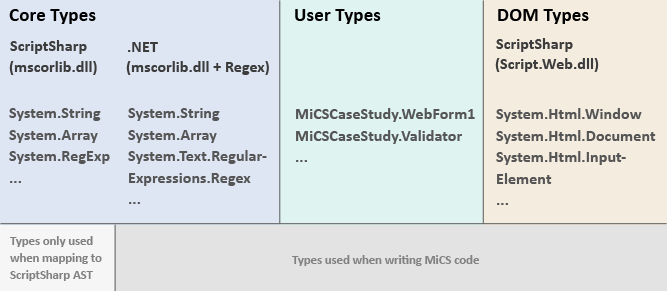
\includegraphics[width=16cm]{resources/images/TypesOverview.png}}
		\end{center}
		\caption{The different types used by MiCS.}
		\label{typesOverview}
	\end{figure}

	Since one of the goals of MiCS is to be able to execute the same code on both client and server side (server client portability) its required that the .NET core types are used when writing MiCS code. This is in contrast to how Script\# works in its original manner where the Script\# core types (that reflect the equivalent JavaScript types) are used. This has some benefits but is also an obstacle that prevents server client portability.

	\subsection{Core Types} % (fold)
	\label{sub:core_types}
		To build the ScriptSharp AST correctly the ScriptSharp core types are required to be associated to the AST nodes. One reason the ScriptSharp core types are required is that they define their equivalent script name (in the class attributes) that is used by the ScriptSharp script generator. An example is the System.Char (see figure \ref{char}) type which is converted to the JavaScript String type as no JavaScript Char type exists.

	\begin{figure}[H]
			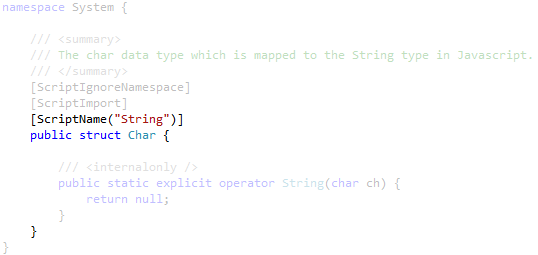
\includegraphics[width=13cm]{resources/images/Char.png}
		\caption{The core type System.Char defined in the Script\# mscorlib.dll.}
		\label{char}
	\end{figure}

		MiCS uses the regular .NET core types when a developer is writing MiCS code but when generating the client side script the Script\# defined core types are used. This implies that some kind of mapping between the two kinds of core types are required. This mapping of core types is explained in section \ref{sub:type_mapping}.
	% subsection core_types (end)

	\subsection{User Types} % (fold)
	\label{sub:user_types}
		User types are the types that are defined by the developer. The user types considered here are either MixedSide types or ClientSide types (i.e. types that have method members that have the either the MixedSide attribute or the ClientSide attribute on them). User type definitions is what the generated client side script eventually will consist of. 

		Pure server side types are obviously also user types but they are not relevant in a MiCS context as JavaScript will not be generated from them.
	% subsection user_types (end)

	\subsection{DOM Types} % (fold)
	\label{sub:dom_types}
		Document Object Model (DOM) types are Script\# infrastructure defined in the System.Html namespace (Script.Web.dll). These classes that represent DOM objects from the browser. The purpose of these classes is only to represent the interface of the actual DOM types in the browser. This is also seen if one looks at the implementation of these types as all their methods and properties on these types return null or false. Like the Script\# core types, DOM types also has their script names in the attribute [ScriptName]. The DOM types are only meant for ClientSide code.

		\begin{figure}[H]
				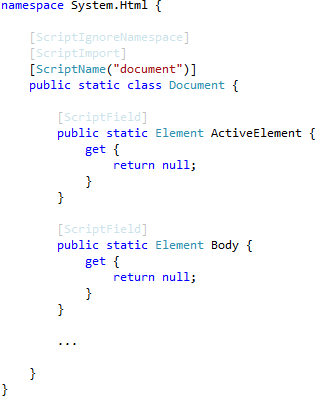
\includegraphics[width=7cm]{resources/images/Document.png}
			\caption{Script\# definition of the DOM type Document.}
			\label{fig:document}
		\end{figure}
	% subsection dom_types (end)

% section types_in_mics (end)